\documentclass[border=4pt]{standalone}
\usepackage[T1]{fontenc}
\usepackage{amsmath}
\usepackage{tikz}
\usetikzlibrary{arrows.meta, shapes.geometric, fit, backgrounds, calc}

\begin{document}
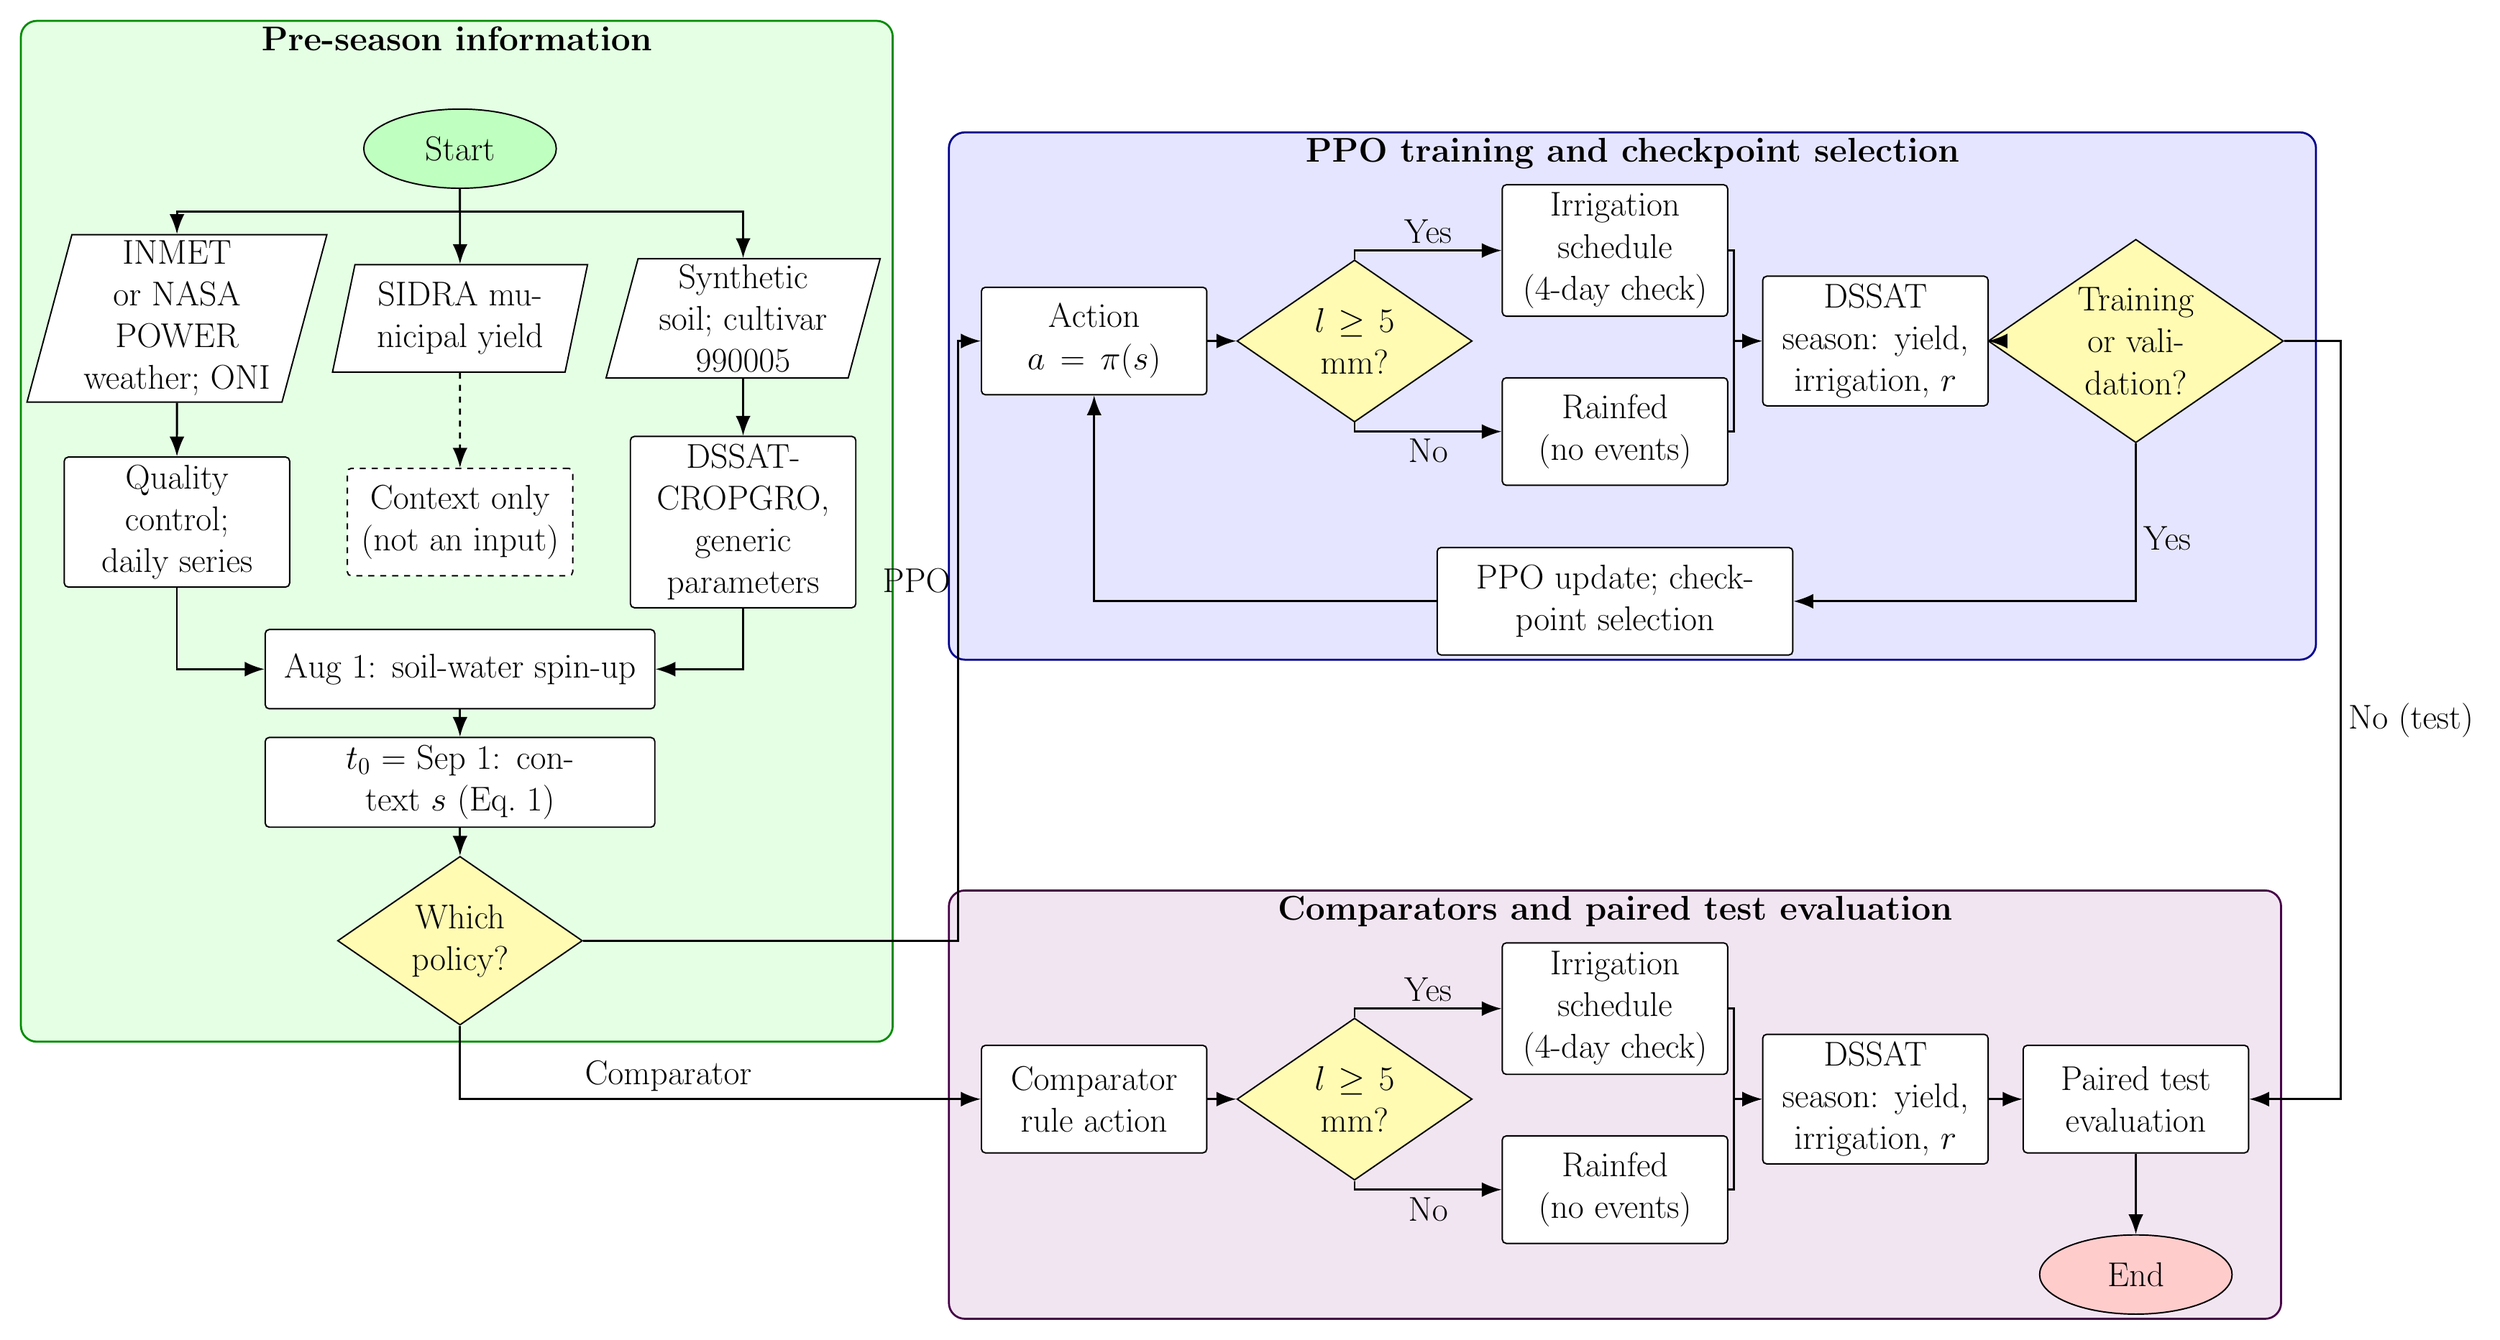
\begin{tikzpicture}[
    x=1cm, y=1cm,
    font=\fontsize{18}{21}\selectfont,
    every node/.style={align=center},
    box/.style={rectangle, rounded corners=2pt, draw=black, line width=0.7pt, text width=3.7cm, minimum height=1.9cm, inner sep=4pt, fill=white},
    data/.style={trapezium, trapezium left angle=75, trapezium right angle=105, trapezium stretches body, draw=black,
                 line width=0.7pt, text width=3.5cm, minimum height=1.9cm, inner sep=3pt, fill=white},
    dec/.style={diamond, aspect=1.45, draw=black, line width=0.7pt, text width=2.3cm, inner sep=1pt, fill=yellow!30},
    term/.style={ellipse, draw=black, line width=0.7pt, minimum width=3.4cm, minimum height=1.4cm, fill=green!25},
    stop/.style={ellipse, draw=black, line width=0.7pt, minimum width=3.4cm, minimum height=1.4cm, fill=red!20},
    arrow/.style={-{Latex[length=3.5mm]}, line width=1pt},
    darrow/.style={-{Latex[length=3.5mm]}, line width=1pt, dashed},
    region/.style={rounded corners=8pt, draw=#1!55!black, line width=1pt, fill=#1!10},
    rtitle/.style={font=\fontsize{18}{21}\selectfont\bfseries, anchor=north}
]

% ------------------------------------------------------------ pre-season block
\node[term] (start)   at (7.4, 0.0) {Start};
\node[data] (weather) at (2.4, -3.0) {INMET or NASA POWER weather; ONI};
\node[data] (sidra)   at (7.4, -3.0) {SIDRA municipal yield};
\node[data] (soil)    at (12.4, -3.0) {Synthetic soil; cultivar 990005};
\node[box] (qc)       at (2.4, -6.6) {Quality control; daily series};
\node[box, dashed] (verif) at (7.4, -6.6) {Context only (not an input)};
\node[box] (cfg)      at (12.4, -6.6) {DSSAT-CROPGRO, generic parameters};
\node[box, text width=6.6cm, minimum height=1.4cm] (spin) at (7.4, -9.2) {Aug 1: soil-water spin-up};
\node[box, text width=6.6cm, minimum height=1.4cm] (t0)   at (7.4, -11.2) {$t_0$ = Sep 1: context $s$ (Eq.~1)};
\node[dec] (which) at (7.4, -14.0) {Which policy?};

% ------------------------------------------------------------ PPO block
\node[box] (genA)  at (18.6, -3.4) {Action $a=\pi(s)$};
\node[dec] (depA)  at (23.2, -3.4) {$l \geq 5$ mm?};
\node[box] (schA)  at (27.8, -1.8) {Irrigation schedule (4-day check)};
\node[box] (rfA)   at (27.8, -5.0) {Rainfed (no events)};
\node[box] (dsA)   at (32.4, -3.4) {DSSAT season: yield, irrigation, $r$};
\node[dec] (split) at (37.0, -3.4) {Training or validation?};
\node[box, text width=6.0cm] (upd) at (27.8, -8.0) {PPO update; checkpoint selection};

% ------------------------------------------------------------ comparator block
\node[box] (genC)  at (18.6, -16.8) {Comparator rule action};
\node[dec] (depC)  at (23.2, -16.8) {$l \geq 5$ mm?};
\node[box] (schC)  at (27.8, -15.2) {Irrigation schedule (4-day check)};
\node[box] (rfC)   at (27.8, -18.4) {Rainfed (no events)};
\node[box] (dsC)   at (32.4, -16.8) {DSSAT season: yield, irrigation, $r$};
\node[box] (eval)  at (37.0, -16.8) {Paired test evaluation};
\node[stop] (end)  at (37.0, -19.9) {End};

% ------------------------------------------------------------ pastel backgrounds
\begin{scope}[on background layer]
  \node[region=green, fit=(start)(weather)(soil)(which)(t0), inner xsep=14pt, inner ysep=26pt, yshift=18pt] (bgA) {};
  \node[region=blue, fit=(schA)(genA)(split)(upd), inner xsep=16pt, inner ysep=14pt, yshift=12pt] (bgB) {};
  \node[region=violet, fit=(genC)(eval)(end)(schC)(rfC), inner xsep=16pt, inner ysep=14pt, yshift=12pt] (bgC) {};
\end{scope}
\node[rtitle] at (bgA.north) {Pre-season information};
\node[rtitle] at (bgB.north) {PPO training and checkpoint selection};
\node[rtitle] at (bgC.north) {Comparators and paired test evaluation};

% ------------------------------------------------------------ arrows: pre-season
\draw[arrow] (start.south) -- ++(0,-0.4) -| (weather.north);
\draw[arrow] (start.south) -- ++(0,-0.4) -| (soil.north);
\draw[arrow] (start) -- (sidra);
\draw[arrow] (weather) -- (qc);
\draw[darrow] (sidra) -- (verif);
\draw[arrow] (soil) -- (cfg);
\draw[arrow] (qc.south) |- (spin.west);
\draw[arrow] (cfg.south) |- (spin.east);
\draw[arrow] (spin) -- (t0);
\draw[arrow] (t0) -- (which);

% decision on the policy
\draw[arrow] (which.east) -- (16.2, -14.0) |- node[left, pos=0.3] {PPO} (genA.west);
\draw[arrow] (which.south) |- node[above, pos=0.7] {Comparator} (genC.west);

% ------------------------------------------------------------ arrows: PPO
\draw[arrow] (genA) -- (depA);
\draw[arrow] (depA.north) |- node[above, pos=0.75] {Yes} (schA.west);
\draw[arrow] (depA.south) |- node[below, pos=0.75] {No} (rfA.west);
\draw[arrow] (schA.east) -| ($(dsA.west)+(-0.5,0)$) -- (dsA.west);
\draw[arrow] (rfA.east) -| ($(dsA.west)+(-0.5,0)$) -- (dsA.west);
\draw[arrow] (dsA) -- (split);
\draw[arrow] (split.south) |- node[right, pos=0.3] {Yes} (upd.east);
\draw[arrow] (upd.west) -| (genA.south);
\draw[arrow] (split.east) -- ++(1.0,0) |- node[right, pos=0.25] {No (test)} (eval.east);

% ------------------------------------------------------------ arrows: comparators
\draw[arrow] (genC) -- (depC);
\draw[arrow] (depC.north) |- node[above, pos=0.75] {Yes} (schC.west);
\draw[arrow] (depC.south) |- node[below, pos=0.75] {No} (rfC.west);
\draw[arrow] (schC.east) -| ($(dsC.west)+(-0.5,0)$) -- (dsC.west);
\draw[arrow] (rfC.east) -| ($(dsC.west)+(-0.5,0)$) -- (dsC.west);
\draw[arrow] (dsC) -- (eval);
\draw[arrow] (eval) -- (end);
\end{tikzpicture}
\end{document}
